\documentclass[12pt]{book}
\usepackage[utf8]{inputenc}
\usepackage[english]{babel}
\usepackage{setspace}
\usepackage{apacite}
\usepackage{amssymb}
\usepackage{amsmath}
\usepackage{float}
\usepackage{array}
\newcolumntype{M}[1]{>{\centering\arraybackslash}m{#1}}
\newcolumntype{N}{@{}m{0pt}@{}}
\usepackage{graphicx}
\usepackage{adjustbox}
\usepackage{enumerate}
\usepackage{algorithm}
\usepackage{algorithm,algpseudocode}
\newcommand\tab[1][1cm]{\hspace*{#1}}
\graphicspath{ {images/} }
\begin{document}
\title{Spelling Correction for Filipino using Double Metaphone and Levenshtein Distance}
\author{Joanna Marie Ompoc and Mikee A. Villanueva}
\date{\today}
\maketitle
\let\cleardoublepage\clearpage
\pagebreak
\tableofcontents
\let\cleardoublepage\clearpage
\listoffigures
\let\cleardoublepage\clearpage
\listoftables
\let\cleardoublepage\clearpage
\chapter{Introduction}
\doublespacing
\section{Research Description}\label{intro}
To use a word also means to spell it correctly. According to \cite{gredler2002snow}, spelling is important in order to fluently read. This is because spelling and reading follows the same mental representation of a word. Learning how to spell means learning information about the word’s print, speech sounds, and meaning\cite{moats2005spelling}. Content writing involves both spell checking and proofreading, and in order for writers to reduce their time in writing, they often forget these important features. Spelling errors on published works may lead to readers not being able to understand the content of your work and they may lose their interest in reading your work because of all the distractions within the content itself. Sometimes, poor spellers tend to only use words that they can spell in their writings. This leads to the lack of verbal power and their work may only focus on the spelling rather than the content itself\cite{moats2005spelling}.

Spelling errors are sometimes caused by hitting the wrong key on the keyboard, cognitive errors like phonetics, and OCR errors which is generally caused by visual similarity. Phonetic errors poses a greater problem in solving spelling errors because these misspellings often have more than a single insertion, deletion or substitution error \cite{kukich1992techniques}. Phonetic spell checkers often use Soundex, originally used for coding and indexing family names, for generating spelling suggestions. Through soundex, any words can be compressed to just a 4-digit code - the first letter of the word follow followed by 3-digit numbers. Spelling correctors often have very large dictionary data thus ways to compress these data must be done so that the dictionary won’t take up too much space \cite{zobel1995finding}. Soundex, however, often produces inefficient spelling suggestions because of its limited code combinations \cite{zobel1996phonetic}. Another method used in phonetic spell checkers is called Metaphone, an improvement to Soundex, which encodes words according to how it sounds. Also, another extension to Metaphone is the Double Metaphone which produces both primary and secondary codes whereas metaphone only produces one\cite{philips2000double}.

Various techniques are used in ranking suggestions like Wagner and Fischer’s sting-to-string correction problem (1974), Boyer-Moore’s fast string matching (1977), Knuth’s fast pattern matching (1977), Sellers’s evolutionary distances (1980), and Levenshtein’s self-correcting codes \cite{blank2012spelling}. The string-to-string correction problem is used to figure out the difference between two strings by using the minimum cost sequence of operations in order to transform one string into the other\cite{wagner1974string}. Boyer-Moore’s fast string matching algorithm finds the location of a string on another string\cite{boyer1977fast} while Knuth’s fast pattern matching algorithm determines how many times a string appears within a string with a run-time that depends on the length of each string\cite{knuth1977fast}. The evolutionary distance method determines the pattern of similarities between two strings\cite{sellers1980theory}. Lastly, Levenstein’s self-correcting codes that calculates the smallest possible insertion, deletion, and substitution to transform one string to the other\cite{levenshtein1966binary}.

A Filipino spellchecker by \cite{cheng2007spellchef} called SpellCheF which is composed of modules such as dictionary-lookup, n-gram analysis, Soundex, and character distance measurements. SpellChef used two methods for generating suggestions - Tri-gram analysis and Soundex. These suggestions were ranked by using character distance method which uses a Pythagorean-type metric. The results showed that more suggestions are generated by using the Soundex approach. However, the tri-gram approach produces more concise suggestions faster than Soundex.

Filipino may almost be the same as Tagalog but it contains “western” letters like f, j, c, x and z.  (“Tagalog Lang”, 2002). Filipino can be referred as a subset of Tagalog because it includes contributions of languages other than Tagalog. Also, foreigners favors “Tagalog” than “Filipino”, and some overseas Filipinos tend to follow what word the foreigners considers more \cite{Filipino}. The phonetic rules for the Double Metaphone will be based from the Komisyon sa Wikang Filipino or KWF’s “Ang Ortograpiya ng Wikang Pambansa”.

This study aims to create a Filipino spelling corrector that will focus on the phonetic structure of each words. Two databases will be utilized for the Filipino dictionary and for the common words dictionary. The Filipino dictionary will contain over 21,000 words which will be retrieved from [https://github.com/jmalonzo/tl-wordlist], a GNU licensed dictionary originally used for Aspell.

Furthermore, the study will be using Double Metaphone to produce spelling suggestions, and Levenshtein Distance to rank the generated suggestions. Then, the results from the aforementioned methods will be memoized to avoid recursions. Each words in the dictionary will be transformed into their Double Metaphone encodings and they will be grouped according to their encodings. The input will also be converted into the encoding and will be matched in the common words dictionary first before the Filipino dictionary. The edit distance of each of the suggestion from the input will be determined using the Levenshtein Distance algorithm and only a maximum of 10 suggestions will be shown to the user.

\section{Statement of the Problem}
Most of word processing programs provides spelling checker and corrector to insure the correctness of their work. Without using any methods we mentioned in Section ~\ref{intro}, the traditional way to detect error and correct those errors is to compare the given text in every words in the dictionary and on the condition that the given text is not found in the dictionary, the given word will then be considered as a misspelled word. Assuming that the given text is misspelled, the system still need to retrieve the correct word of the text. However, deciding which word is correct can be a challenge for the system since the misspelled word may have several possible correct words. Furthermore, having such a big dictionary can cause a slower running time to the system resulting to a slower program, and aiming suggestions accuracy is also a challenge. 

\section{Research Objectives}
\subsection{General Objectives}
To provide a Spelling Corrector for Filipino using the Double Metaphone and Levenshtein Distance.
\subsection{Specific Objectives}

\begin{enumerate}
  \item	To create phonetic rules using the manual entitled “The Filipino Orthography” from the KWF or Komisyon sa Wikang Filipino.
  \item	To provide spelling suggestion using Double Metaphone
  \item	To provide ranking for the suggestions using the Levenshtein Distance.
  \item	To utilize the memoization technique for faster retrieval of data from the \textit{commonwords} database.
	\item to compare the performance using the metaphone and levenshtein method and using the levenstein method. 
	\item To evaluate the performance of the system on its ability to check spelling and provides suggestion for misspelled words.

\end{enumerate}

\section{Scope and Limitation of the Study}
Document files, that are encoded in .txt format, in Filipino language will be used as test subjects in this study. The study only limits the use of text files instead of documents that contain images, tables and graphs. Furthermore, this study focuses on generating spelling suggestions rather than the detection of misspellings within the document.

\section{Significance of the Study}Spelling checker for Filipino language is significantly important especially for Filipino, since it can help further development and enrichment of native languages such as Hiligaynon, Chabacano, Cebuano, and other different language in the Philippines. Furthermore, spelling corrector also plays a significant role in learning a language, thus having this study may help other individuals in learning the Filipino language. This study also creates the metaphone rules for Filipino Language which are beneficial for researchers with a similar study.

\let\cleardoublepage\clearpage
\chapter{Review of the Related Literature}
The topics that are included in this chapter helps to gain information that are relevant and similar to the present research. The topics below includes discussions on Spell Checker, Phonetic Matching, Levenshtein Distance, and Memoization.

\section{Spell Checker}
\subsection{Filipino Spell Checking and Correction}
SpellCheF is a Filipino spell checker that uses dictionary-lookup, n-gram analysis, Soundex, and character distance measurement for the detection and correction of misspelled words \cite{cheng2007spellchef}. 
The spell checker is composed of the lexicon builder module, n-gram analysis module, detection module, and correction module. The extraction of each words from the source materials is located at the lexicon builder module. These words will be categorized according to the rules from KWF rulebooks, the 2001 Revision of the Alphabet and Guidelines in Spelling the Filipino Language, and the Gabay sa Editing sa Wikang Filipino. In the n-gram analysis, the system executes a non-positional tri-gram analysis where three n-gram look-up tables will be generated. These tables contains the KWF lexicon, Gabay lexicon, and the Common Words lexicon. The detection module’s work is to decide whether a word is correctly spelled or misspelled. Since the system is a plug-in to OpenOffice Writer, this module will be called on this software. Then, it is in the corrector module where suggestions will be generated. This module utilizes both Soundex code and Tri-gram Analysis. Finally, after generating the list of correct spelling suggestions, these words will be ranked by using character distance method which is used to arrange and trim the suggestions. To rank the suggestions from the aforementioned method, the Pythagorean-type metric was used to determine the edit distance between the misspelled word and a suggestion.

According to their result, the Corrector module achieved a 94\% accuracy rate while their Detector module achieved an error rate of 7\% which means that some correct words were flagged as misspelled. Reasons for this error are small lexicon, low frequency of the tri-gram, and two-letter words that are not included in the lexicon. Also, the length of the misspelled word and the suggestions greatly affect the rank of the suggestions because when the suggested word and the misspelled word has the same length, then that suggestion will appear on top of the list.

Furthermore, according to their results on the suggestion module, even though Soundex produced more suggestions than the tri-gram approach, produced more efficient suggestions than Soundex. This is because Soundex always accepts the first letter of every word as correct.

\subsection{Afrispel: An isiZulu Spell Checker}
Another spell checker for an African language uses an algorithm where it will take in an input text which will be tokenized and then it will search for these words in the exception list. The words are then individually searched in the exception list that is collected from the corpus. The exception list contains known correctly spelled words. This will help minimize the number of words to be taken through the error detection algorithm. The words that are not on the exception list, referred to this study as the non-word errors, will be taken to the error detection algorithm. For detecting non-word errors, the researchers used the combination of the character-trigrams or character-four-grams and the probability of having each character-trigram or four-gram in a particular training dataset. The researchers also used a hash table for the exception list because it is fast and it minimizes the number of comparisons for the lookup \cite{ndabaafrispel}.

The system’s spell checker has a high accuracy rate when detecting words that are not in the training sets. The three corpora that are used in the n-gold cross validation also achieved a high-performance rate. The Ukwebalana corpus, which achieved the highest result, had an accuracy rate of 85\% with a threshold of 0.003, Prof. Langa corpus had an accuracy rate of 67\% at 0.003, and finally, the news items corpus achieved an accuracy of 76\% with 0.003 thresholds. However, testing the system with an outdated corpus can lead to a poor performance where Ukwebalana had 50\% accuracy rate. This shows that a spell checker’s performance highly depends on its corpus. Furthermore, the spellchecker performed better with trigrams compared with four-grams because it is most likely to find trigrams of a word than its four-grams.

Although their study doesn’t include suggestions, according to the researchers, the error detection of the system is their first priority. Also, the spell checker flags infrequent words as wrong spelling. The researchers suggest an improvement in the data-driven statistical language model with a theory-driven linguistic model when building a spell checker. With this, the spell checker would be able to check if an infrequent word follows the language rules, and this may improve the system’s performance. Lastly, a spell checker should also be able to detect unlikely combinations of words.

\subsection{GNU Aspell}
An Open source spell checker called GNU Aspell can be used as a library or a standalone spell checker \cite{atkinson2016}. It is specially designed to replace Ispell - a program that can correct spellings and typographical errors in any files \cite{ispell}.  Aspell does the best word suggestion replacements for misspelled word for the English language, it can easily check documents in UTF-8 without using a special dictionary, it also includes support for multiple dictionaries at once, and it can handle personal dictionaries when multiple Aspell process is open at once \cite{atkinson2016}. Aspell’s process, as described by \cite{atkinson2004}, is listed below:
\begin{enumerate}
	\item The misspelled words will be converted to the correct word with almost the same sound.
	\item It lists all words that sounds alike with only one or two edit distance from the source word. When it is set to only look for words with only one edit distance, it will compare it to all possible words that sound alike, and each words will be checked in the dictionary. But when two edit distance is to be found, it will scan the whole dictionary, and it will pick up all suggestions. The spell checker is fast because it limits only until two edit distance.
	\item It will then find common misspelled words that have the same correct spelling replacement and store it in the same suggestion list as if it was a correct spelling.
	\item The suggestions will be ranked and the suggestion with the lowest score will be returned.
	\item Lastly, the correctly spelled word will be replaced to the misspelled word.

\section{Phonetic Matching}	
\subsection{SoundEx}
A study by \cite{stanier1990accurate} used statistical tests into a couple of data sets which contains 411,716 surnames to establish the accuracy of Soundex coding. According to Alan, only a third of the matches that will be found are correct but a quarter of correct results won't be discovered. The results of his study shows that only 33\% of the Soundex results are correct and the 25\% genuine matches that were not located was the major problem. According to Stanier, the shorter the code, the higher the number of incorrect matches will be found because given surname pairs like \textit{Cholmondely} and \textit{Chumley}, both surnames will be variants of the same soundex code but \textit{Askey} and \textit{Haskey}, and \textit{Lloyd} and \textit{Floyd} won't even be a match.

According to \cite{christian1998soundex}, the following principles are the three main principles used in creating Soundex rules:
\begin{enumerate}
	\item Sometimes, the features of some surname contains too many variable and it is hard to be coded efficiently. Vowels are important in the English dialect variation, and it is hard to create an easy and efficient vowel-coding scheme that includes obvious variants. However, single or double consonants may be highly variable but they are not very significant.
	\item There are letters that sounds alike but treated individually. Variants like 'd' and 't' sounds alike and can be interchanged because they are identified as "dental stops" for the English language.
	\item Letters that are used differently, and letters that are used because they sound alike are coded in one group. The letter 'g' can be used for both 'g' and 'j', and the letter 'c' can be used for 's', 'k', and 'ch'. These two letters with their corresponding sound alike are coded into a single large group.
\end{enumerate}

However, there are two fundamental principles of spelling that are ignored in Soundex. These principles listed below are very important in the English language:
\begin{enumerate}
	\item There are some combination of letters that represent a single sound. 'dg' (sometimes spelt as 'j') is one sound and not a combination of the single letters 'd' and 'g'. Also, the combinations 'ch' and 'tch' have a similar sound but both are coded by Soundex differently. Thus, it makes 'Bachelor' and 'Batchelor' as matches.
	\item Consonants that are clustered together don't produce one sound, and an easier spelling is reflected on this. The consonant combination 'ndl' in Lindley sounds like 'nl', and thus pronouncing it as Linley. It works the same as Wiltshire to Wilshire, and Christmas to Chrismas.
\end{enumerate}

According to the results of Christian's study, there is a problem with how Soundex code starts with the first letter of the word, and the way it ignores vowels. This may produce misunderstandings, because \textit{Askey} is A200, and \textit{Haskey} is H200. Possible improvements for Soundex should include the addition of "\textit{single letter}" rules where, initial letters should be ignored, all initial vowels should be coded to single codes, or finals consonants should be dropped.


\subsection{Double Metaphone}
A study by \cite{yacob2004application} that uses Double Metaphone algorithm for the correction of Amharic orthography. Amharic orthography follows the rule "if a word sounds right when read aloud then it was rightly written". However, errors encountered on the Amharic spelling includes erros that are inherent from symbol redundancy, phonology-orthography disconnect, foreign language transcription, and typing system.

In the study, before implementing the metaphone algorithm for Amharic, Figure ~\ref{amharic} conversion rules were created for the algorithm to be insensitive to the distinction between symbols but instead of sound.

\begin{figure}
\begin{center}	
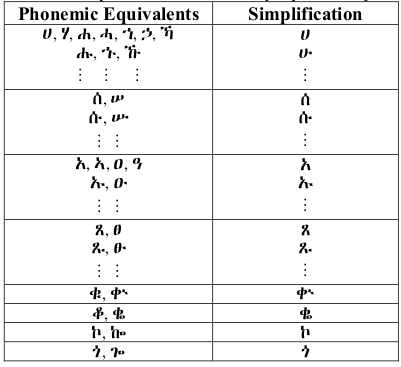
\includegraphics[scale=.65]{amharic.png}
	\caption[Simplification of Phonetically Equivalent Syllables]
	{ Simplification of Phonetically Equivalent Syllables}	
	\label{amharic}
\end{center}
\end{figure}
	
\end{enumerate}

On the double metaphone algorithm, two phonetic encodings will be generated were the frist encoded word is the most probable representative of the target word while the second encoded word serves as an alternative under frequenty used English words. However, this study will limit more than two encodings because according to the researchers, many encodings might appear useful under Amharic writing conventions.

The study’s Amharic metaphone algorithm was compared with the double metaphone algorithm with the same training sets. The gathering of the sample words was converted into an english representation so that the double metaphone can be applied. This method may affect the accuracy of the Double Metaphone.

The results at Figure ~\ref{amharicresults} shows that the Amharic Metaphone achieved the highest accuracy rate amongst the another methods.

\begin{figure}
\begin{center}	
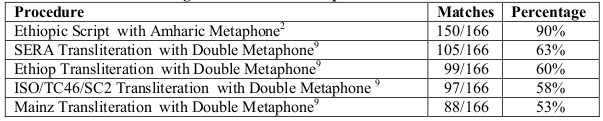
\includegraphics[scale=.65]{amharicresults.png}
	\caption[Words Matching Results for 166 Mispelled Forms of 116 Words]
	{Words Matching Results for 166 Mispelled Forms of 116 Words}	
	\label{amharicresults}
\end{center}
\end{figure}


It is evident from the limited test conducted that higher matching rates are found for Amharic words when the Metaphone algorithm is adjusted to apply the rules of Amharic orthography in lieu of those of English. This positive result has held up as the test set of words has grown in number, a trend that is expected to continue. However, a much more thorough test with a larger corpus of materials should certainly be conducted.

Ultimately any approach to Amharic spelling correction is limited by the reliability of the reference used for canonical formations. The establishment of a comprehensive and authoritative lexicon for written Amharic would be the single most valuable resource towards the realization of this eventual goal.


\section{Levenshtein Distance}
A study of biological sequences using the Damerau-Levenshtein distance uses linear space algorithm to compute the distance between two strings and to find edit operation sequences. Their algorithm requires O(s min{m,n} + m + n) space whereas previous algorithm require O(mn) space. They have also developed a cache efficient and multi-core linear-space algorithm where the cache efficiency was analyzed using a simple cache model \cite{zhao2017efficient}.

A study by \cite{hicham2012introduction} present a new approach dedicated to correcting the spelling errors of arabic language. The method of the study is inspired from levenshtein algorithm and allows a finer and better scheduling than Levenshtein. The study modified the levenshtein distance between two words by taking into account the following matrices: 

\begin{enumerate}
	\item Matrix frequency of insertion error.
	\item Matrix frequency of deletion error.
	\item Matrix frequency of permutation error.
\end{enumerate}

The result shows that compared to levenshtein, out of 190 erroneous words levenshtein  has only 19 classified in the first position while the new approach correctly classified 119 words in the first position. the rest of 119 was distributed on the 2nd, 3rd, 4th, 5th .. 10th position. Statistically the study’s method has proposed 62.63\% of correct words  in the first position against 10\% for levenshtein. 

Another Study by \cite{sarveswaran2015hierarchical} integrated existing approach and new approach such as rule-base, crowdsourcing and suggestions generation using character level n-gram for spelling checker of Tamil language. In the proposed approach the levenshtein distance check each word in the dictionary whether it matches and flag the misspelled, the n-gram based technique is then used to generate possible suggestion of the misspelled word.  250,000 unique error-free words  are included in their dictionary that have been collected in various sources using crowdsourcing, since it is very difficult to gather all words in Tamil Language. Required rules are written to get the appropriate suggestion by considering Canti check as well to identify the appropriate joining letter of two adjoined words. Furthermore, To reduce the search space, the dictionary  has been divided into different files based on the first letter of the word.  The result shows 85.77\% accuracy when considering the suggestion generation. This result had been calculated by analysing the suggestions generated by the system for the words that are not in the dictionary.

\section{Memoization}
A study by \cite{johnson1995memoization} shows how constraints can be propagated using a memoizing parser in the same way as variable binding since some linguistic constraints cannot be all resolved during parsing at the location where they were naturally introduced. The study involves formalizing their approach to memoization and constraints within the general theory of Constraint Logic Programming (CLP) by Hohfeld and Smolka (1998). They also discussed how their method can be applied to a more standard chart parsing. Furthermore, their study extends the previous work of Dorre and Johnson by generalizing the methods used to arbitrary constraint system, which includes feature-structure constraints.

Another study by \cite{johnson1995memoizationj}, used memoization by defining a higher-order procedure memo which takes a function as an argument and returns a memoized version of it. This method stores the memo table as an association list resulting in a less than optimal implementation. Optimal performance would be probably by encoding string positions with integers in the parsing context allowing memo table look-up to be a single array reference.

A new technique by \cite{frost2003monadic}, enables a systematic and selective memoization of a wide range of algorithms. This technique can overcome disadvantages of previous approaches. This technique can help programmers avoid mistakes which can result in suboptimal use of memoization. The resulting memoized programs were amenable to analysis by using equational reasoning. According to Frost’s study, the programmers will be provided with a function memoize which can be used to \textit{memoize} selected parts of  a program. When the \textit{memoized} parts of the program is executed then the function memoize will take care of updating and using the memo tables.


Most of the study that uses large lexicon produces higher percentage of accuracy and low percentage of error rate this shows that most of the spelling checker depends on the lexicon used however 
SoundEx produces many suggestion words but most of this suggestion are inefficient because of many possible suggestions using the code.
 Also, most of the spelling checkers uses N-grams in producing suggestions because of its accuracy but the lengths of the words in the dictionary must always be considered when choosing what N-gram will be used - bi-gram, tri-gram, four-gram, or five-gram.


\let\cleardoublepage\clearpage
\chapter{Theoretical Framework}
The discussion below includes topics on Natural Language Processing, Metaphone, Levenshtein Distance, and Memoization. These discussions help readers to understand the terms that are used in this study.

\section{Natural Language Processing}

According to \cite{chowdhury2003natural}, Natural Language Processing or NLP is the area of research that explores how computers are used to understand and manipulate natural language texts so that it can do useful things. 

Another definition states that NLP is the computerized approach to analyzing texts that are based on both sets of theories and sets of technologies \cite{liddy2001natural}.

Researchers in NLP aim to gather information on how human beings understand and use language so that there will be appropriate tools and techniques will be developed to make computer systems understand and manipulate natural language to perform desired tasks. Machine translation, natural language text processing and summarization, user interfaces, multilingual and cross language information retrieval (CLIR), speech recognition, artificial intelligence and expert systems, and many more are only some of the applications of NLP \cite{chowdhury2003natural}.

\section{Metaphone}
Metaphone is an english phonetic algorithm published by Lawrence Philips in 1990. Metaphone processor represent the string value into a code based on its pronunciation. The processor allows to specify the maximum length of the Metaphone code (up to a maximum of 12 characters). An example shown at Figure ~\ref{metaphone} transform the NAME attribute with the use of default maximum length of 12 characters.

\begin{figure}
\begin{center}	
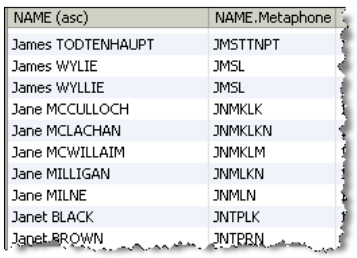
\includegraphics[scale=.50]{metaphone.png}
	\caption[Metaphone]
	{Metaphone}	
	\label{metaphone}
\end{center}
\end{figure}

Lawrence Philips later on produce a new version of metaphone called Double Metaphone. It is called "Double Metaphone" because it returns a both a primary and a secondary code for a string.

\section{The Filipino Orthography}
In pronouncing borrowed words or "Hiram na Salita" from its original spelling the following rules should be followed:

\subsection{Maintaining the structure of the original word}
The letters, both vowels and consonants, can represent more than one sound, for example:

\begin{enumerate}
\item \textbf{'c' - 'k', 's', or 'č'.} “casa” = ('ka.sa), “cello” = ('če.low), and “ice” = ('?ays).
\item \textbf{'j' - 'h'.} “jack” ('jak), and “jai alai” ('hay ?a.'láy)
\item \textbf{'x' - 's', or 'ks'.} “extra” ('?eks.tra), and “xylophone” = ('say.lo.fown).
\item \textbf{'f' - 'p'.} “father” - ('pa:.der)
\item \textbf{'v' - 'b'.} “visa” (vi.sa) - (bi.sa) 
\item \textbf{'z' - 's'.} “zoo” (zu) - (su) 
\item \textbf{'æ' - 'a'.} “map” (mæp) - (map)
\item \textbf{'ow' - 'o'.} “goal” (gowl) - (gol)
\item \textbf{'i:' - 'i'.} “brief” (brif) - (brip)
\item \textbf{'u:' - 'u'.} “shoot” (šut) - (šut)
\end{enumerate}

\section{Levenshtein Distance}
Levenshtein Distance between two strings is the minimal number of insertions, deletions, and substitutions of one character for another that will transform the source string into the target string. The distance is the number of deletions, insertions, or substitutions required to transform the source string into the target string. The Minimum Edit Distance uses sequence of edits represented by Figure ~\ref{minedit}.
\begin{figure}[H]
\begin{center}	
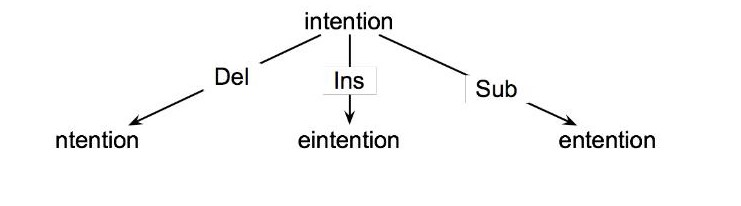
\includegraphics[scale=.50]{minedit.jpg}
	\caption[Minimum Edit Distance]
	{Minimum Edit Distance}
	\label{minedit}
\end{center}
\end{figure}

The greater the Levenshtein distance, the more different the strings are. Furthermore, the Levenshtein Distance Algorithm has been used in Speech Recognition, Plagiarism Detection and Spell Checking. %\cite{Levenshtein}


\section{Memoization}
The term "memoization" was introduced by Donald Michie in the year 1968. It's based on the Latin word memorandum, meaning "to be remembered". It's not a misspelling of the word memorization, though in a way it has something in common.

Memoization is a technique used in computing to speed up programs. This is accomplished by memorizing the calculation results of processed input such as the results of function calls. If the same input or a function call with the same parameters is used, the previously stored results can be used again and unnecessary calculation are avoided. In many cases a simple array is used for storing the results, but lots of other structures can be used as well, such as associative arrays, called hashes in Perl or dictionaries in Python (Stonelen, 2006).

In this study, when the same word occurs again in the document the system will no longer need to check if this input data is valid word or invalid word instead the system will called the data store by memoization.

\let\cleardoublepage\clearpage
\chapter{Methodology of the Study}

In this chapter, the following are discussed: Conceptual Framework, Data gathering, Storing Data to Database, Spell Checker, Spell Corrector, Postprocessing, Evaluation and the Tools and Technology.

\section{Conceptual Framework}
The will system have five stages - preprocessing, dictionary lookup, extracting suggestions, postprocessing and evaluation. First, the \textit{preprocessing of the dictionary} involves the grouping of all words according to their similar encodings and the \textit{preprocessing of the misspelled word} involves the checking if the input appeared recursively or not, and the conversion of the misspelled word to double-metaphone format referred as \textit{meta-word}. Then, the \textit{dictionary lookup} involves matching the misspelled word to the \textit{Dictionary}. The Dictionary contains double-metaphone formats referred as \textit{code} and their corresponding words with the format \\
\{'code': \big['word1', 'word2', ..., 'wordn'\big]\}. In the \textit{Extract Suggestions Module} module, the matched \textit{code} from the \textit{meta-word} will be retrieved with its corresponding words - the suggestions.  After that, the suggestions will be ranked. A maximum of 10 suggestion will be set and these suggestions can only be displayed. Then in the \textit{postprocessing} stage, there will be a client-side notification so that the user will be able to choose if they want to replace the source word or not. Finally, the system will be evaluated according to its precision. Figure ~\ref{systemarchitecture} illustrates the stages of processing the words in our system.

\begin{figure}
\begin{center}
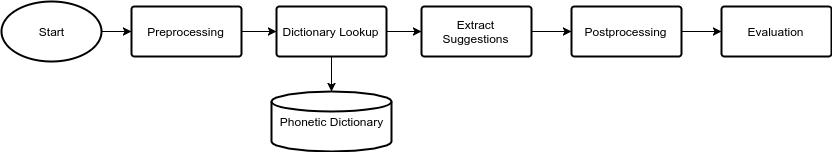
\includegraphics[scale=.50]{systemarchitecture.png}
	\caption[System Architecture]
	{System Architecture}
	\label{systemarchitecture}
\end{center}
\end{figure}

\section{Data Gathering}
The researchers will gather documents that merely consist of texts. The document should only have a maximum number of 250 words. Some of these documents will be gathered from the Filipino Department, College of Arts and Social Sciences. The study will also utilize the data from a Filipino dictionary for Aspell.

\section{Preprocessing}
\subsection{Misspelled Word}
Figure ~\ref{processflowchart_dict} is the visual representation of the process which will be discussed further in this section.

\begin{figure}
\begin{center}	
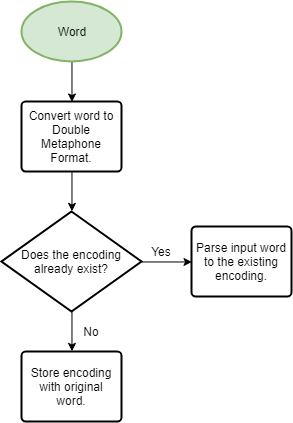
\includegraphics[scale=.60]{preprocessing_dict.png}
	\caption[Process Flowchart of Dictionary Preprocessing]
	{Process Flowchart of Dictionary Preprocessing}	
	\label{processflowchart_dict}
\end{center}
\end{figure}

The data of the dictionary is specifically formatted in the manner where \textit{code} and their corresponding words called \textit{wordn} will be coded into \{'code': \big['word1', 'word2', ..., 'wordn'\big]\}. First, the word will be encoding to its double metaphone format, referred as \textit{code}, where Table ~\ref{phoneticvalues} shows the Metaphone values of each characters based on the Filipino Orthography. Then system will first check if the encoding already exists or not. If the encoding doesn't exists, then the encoding will be stored with the input word in the format  \{'code': \big['word'\big]\}. But if the encoding already exists, then the word will be parsed to the encoding in the format \{'code': \big['word', 'new word'\big]\}.

\begin{table}
\begin{center}
\begin{tabular}{ |c|c| } 
 \hline
 Value & Letters\\
 \hline
 a & 'a', 'e', 'i', 'o', 'u' \\
 \hline
 b & 'b', 'v' \\
 \hline
 c & 's', 'k' \\
 \hline
 d & 'd' \\
 \hline
 f & 'p', 'f' \\
 \hline
 g & 'g' \\
 \hline
 h & 'h' \\
 \hline
 j & 'j', 'h', 'dy' \\
 \hline
 k & 'k','q' \\
 \hline
 l & 'l' \\
 \hline
 ll & 'ly', 'y' \\
 \hline
 m & 'm' \\
 \hline
 n & 'n' \\
 \hline
 Ñ & 'ny' \\
 \hline
 ng & 'ng' \\
 \hline
 p & 'p', 'f' \\
 \hline
 q & 'kw', 'ky', 'k' \\
 \hline
 r & 'r' \\
 \hline
 s & 's' \\
 \hline
 t & 't' \\
 \hline
 v & 'b', 'v' \\
 \hline
 w & 'w', 'ua', 'ue', 'ui', 'oa', 'au', 'ou' \\
 \hline
 x & 'ks', 's' \\
 \hline
 y & 'y', 'ia', 'ie', 'io', 'iu', 'ea' \\
 \hline
 z & 'z', 's' \\
 \hline
\end{tabular}
\caption{Phonetic Values Table} \label{phoneticvalues}
\end{center}
\end{table}

The vowels are only used in the encoding when it is at the beginning of the word and compared to Metaphone, Double Metaphone returns both the primary and secondary code for a string. For example, the letter \textit{K} has two encodings - \textit{K} and \textit{Q}. So, given a word \textbf{kolehiyo}, the system will generate two encodings, \textit{KLHY} as primary and \textit{QLHY} as secondary. Also, given a word beginning with a vowel, \textit{alapaap}, the system will generate the encodings \textit{ALPP} and \textit{ALFF}.

\begin{algorithm}
  \caption{Double Metaphone Algorithm}
	\textbf{DoubeleMetaphone}(s) transforms string \textit{s} of length \textit{k(s)} into the Double Metaphone primary and secondary keys, $t_{1}$ and $t_{2}$ respectively. \\
	The major steps of the algorithm are as follows:
	\begin{enumerate}
	\item Set the phonetic values.
	\item Initialize input string.
	\item Transform input string into its Double Metaphone encoding.
	\end{enumerate}
	We now examine these steps in detail.
	\begin{enumerate}
	\item Set the phonetic values\\
	
	Table ~\ref{phoneticvalues} contains the phonetic rules, denoted as rn, for all 26 letters of the Filipino alphabet, denoted as fm. Where m is the number of the Filipino alphabet, and n is the number of rules in each alphabet.Take note that both rn and fm should in uppercase.
		\begin{enumerate}[(a)]
		\item Set $f_{m}\gets (r_{1}, r_{2}, ..., r_{n})$		
		\end{enumerate}
	the number of rules for every alphabet is len($f_m$) $>=$ 1.	
	\item Initialize input string.\\
	This step normalizes the input string, denoted by s, into its uppercasing.
		\begin{enumerate}[(a)]
		\item input = s
		\item input.upper()
		\end{enumerate}
	\item Transform input string into its Double Metaphone encoding.\\
	To produce the primary and secondary keys, denoted by t1 and t2 respectively, the input string s will first go over a \textbf{while} loop, then a succession of nested \textbf{if-else} loops. Below is the phonetic rule for the letter “B”:
		\begin{enumerate}[(a)]
		\item \begin{algorithmic}
    \If{symbol is “B”}\\
\tab {$t_{1} \gets$ “B” \\
\tab $t_{2} \gets$ “V”\\
\tab Increment current}\\
	\Else \\
	\tab {$t_{1} \gets$ “B” \\
\tab $t_{2} \gets$ “V”\\
\tab Increment current\\
\tab continue}\\
	\EndIf
  \end{algorithmic}
		\end{enumerate}
	\end{enumerate}
\end{algorithm}

\subsection{Misspelled Word}
Figure ~\ref{processflowchart} is the visual representation of the process which will be discussed further in this section.

\begin{figure}
\begin{center}	
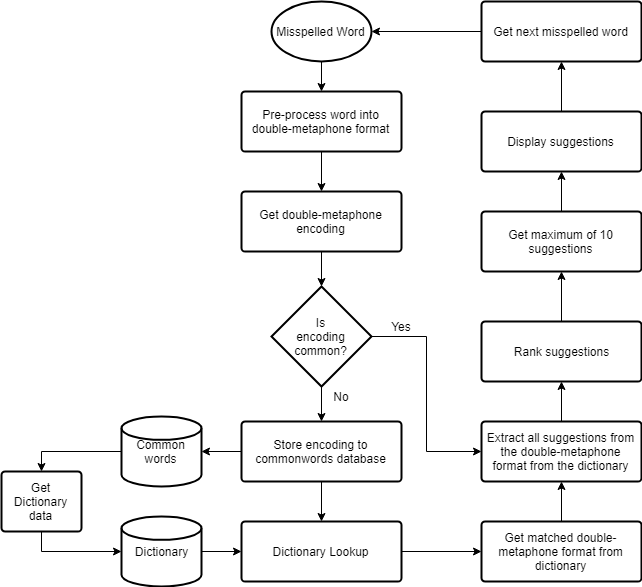
\includegraphics[scale=.60]{processflowchart.png}
	\caption[Process Flowchart of Misspelled  Word Preprocessing]
	{Process Flowchart of Misspelled  Word Preprocessing}	
	\label{processflowchart}
\end{center}
\end{figure}

The \textit{commonwords} database contains the memoized data from the previous input of the system. The memoized data will be removed from the \textit{Dictionary} and it will be transfered to the \textit{commonwords} database since the misspelled word input is first matched in the \textit{commonwords} database and if the misspelled word is not common, then it will be matched to the \textit{Dictionary}.

If the memoized data wont be transfered to the \textit{commonwords} database, then the input will be compared again to (in worst case) more than 50\% of the \textit{Dictionary} data that is already in the \textit{commonwords} database. Thus, this method is necessary.

The \textit{dictionary} and \textit{commonwords} database's data will inputted into the format shown at Figure ~\ref{dictionary}

\begin{figure}
\begin{center}	
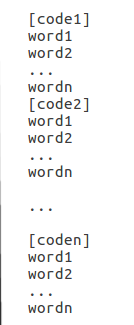
\includegraphics[scale=.60]{dictionary.png}
	\caption[Dictionary Layout]
	{Dictionary Layout}	
	\label{dictionary}
\end{center}
\end{figure}

The misspelled word input will be converted to its double-metaphone format. 

\section{Dictionary Lookup}
The misspelled word, which is in double-metaphone format called \textit{meta-word}, will be matched in the dictionary. If a match is found, then the code with its corresponding word will be retrieved. 

Given a misspelling \textit{qolehiyo}, the encoding that will be generated will be \textit{KLHY} and \textit{QLHY}. The system will retrieve matches for these encoding with its corresponding words from the dictionary.

\section{Extract Suggestions}
The corresponding words of the code on the dictionary will be extracted. These corresponding words will be the suggestions. The suggestions will be ranked by using Levenshtein Distance. After ranking, only a maximum of 10 suggestions will be retrieved.

In finding the edit distance between the source word \textit{qolehiyo} and a target word \textit{kolehiyo}, we will be using the algorithm below where the results are visualized Figure ~\ref{editdistancetable}.

\[
   D(\textit{i,j})= min
\begin{cases}
   D(i-1,j)+1\\
   D(i,j-1)+1\\
   D(i-1,j-1)+1,              & \begin{cases}
   2, & \text{if} S_{1}(i) \neq S_{2}(i)\\
   0, & \text{if} S_{1}(i) = S_{2}(i)
\end{cases}
\end{cases}
\]

\begin{figure}[H]
  \centering
          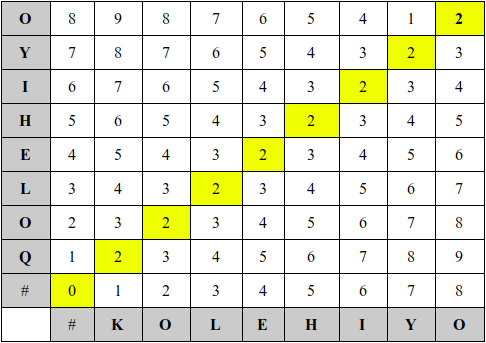
\includegraphics[scale=.60]{editdistancetable}
          \caption{The Edit Distance Table}
          \label{editdistancetable}
\end{figure}


\begin{algorithm}
 \caption{Levenshtein Distance}
	\textbf{LevenshteinDistance}(s,r) determines the edit distance between two string, \textit{s} and \textit{r}, whose lengths are \textit{k(s)} and \textit{k(r)}. The edit distance can be acquired by setting a value for every insertions, deletions, and substitutions. \\
	The major steps of the algorithm are as follows:
	\begin{enumerate}
	\item Initialize the matrix.
	\item Compute the Edit Distance.
	\end{enumerate}
	We now examine these steps in detail.
	\begin{enumerate}
	\item Initialize the matrix.\\
	The matrix will have a \textit{k(s) x k(r)} size. Also, the row and column of the matrix will indexed from 0 to \textit{k(s)} and 0 to \textit{k(r)} respectively.
		\begin{enumerate}[(a)]
		\item Set $matrix\gets [k(s)+1][k(r)+1]$		
		\end{enumerate}
	
	\item Compute the Edit Distance.\\
	Each letters (row-wise, and column-wise) will be compared. If two letters are the same, then the value at index \textit{[x,y]} will be the minimum of the values at index \textit{[x-1, y]+1}, index \textit{[x-1, y-1]}, and index \textit{[x, y-1]+1}. Otherwise, the values at index \textit{[x,y]} is the minimum of the value at index \textit{[x-1, y]+1}, index \textit{[x-1, y-1]+1}, and index \textit{[x, y-1]+1}. After traversing to all letters, the edit distance will be the value at index \textit{[k(s)+1, k(r)+1]}.
	\begin{enumerate}[(a)]
		\item \begin{algorithmic}
      \For{\texttt{$x \gets 1 ... k(s)+1 $}}
      \For{\texttt{$x \gets 1 ... k(s)+1 $}}
    \If{index $[x-1,0] \gets$ index $[0, y-1]$ }\\
     \tab \tab {matrix $[x,y] \gets$ minimum of (
\tab \tab \tab \tab \tab\tab $[x-1, y]+1,$\\
\tab \tab \tab \tab \tab\tab$[x-1, y-1],$\\ 
\tab \tab \tab \tab\tab\tab$[x, y-1]+1$)}
	\Else \\
	\tab \tab { matrix $[x,y] \gets$ minimum of ( \\
\tab \tab \tab \tab \tab\tab $[x-1, y]+1,$\\
\tab \tab \tab \tab \tab\tab$[x-1, y-1],$\\ 
\tab \tab \tab \tab\tab\tab$[x, y-1]+1)$ }
    \EndIf
          \EndFor
      \EndFor
  \end{algorithmic}
   \end{enumerate}
	\end{enumerate}
\end{algorithm}



\section{Postprocessing}
An instance were the \textit{source word} is a noun and flagged as a misspelled word since it is not located in the dictionary. To solve this problem, we propose a \textit{client-side notification} were the user will have to choose whether to treat the \textit{source word} as a \textit{misspelled word} and replace it with the \textit{correct word} or not. If the \textit{source word} is indeed a misspelled word but it is not in the dictionary, then the \textit{source word} will be added to the \textit{commonwords} dictionary along with its corresponding word suggestions.

\section{Evaluation}
In this study the evaluation of spelling checker is based on ISO 9126 standards. For our proposed metrics, we used the Suggestion Measures from the combined the metrics of TEMAA, Starlander \& Popescu-Belis , and Van Zaanen \& Van Huyssteen where we describe the following:

\begin{enumerate}
\item True positives (Tp): valid words recognised by the spelling checker.
\item True negatives (Tn): invalid words recognised by the spelling checker.
\item False negatives (Fn): valid words not recognised by the spelling checker.
\item False positives (Fp): invalid words not recognised by the spelling checker.
\end{enumerate}

\subsection{Suggestion Measures}
According to \cite{van2004re}, suggestion adequacy or SA is the spelling checker's ability to produce relevant suggestions for all incorrect words that are flagged by the spelling checker or the true negatives. The SA of a spelling checker should only be based on true negatives, and not on all negatives, since the aim is to determine how well the spelling checker can suggest corrections for incorrect words.

The following scoring system is derived from Paggio \& Underwood, and Van Zaanen \& Van Huyssteen’s scoring system:
\begin{enumerate}
\item Correct suggestion is the first suggestion = 1 (CS 1 ).
\item Correct suggestion is a visible suggestion = 0.5 (CS 2 ).
\item All corrections are incorrect = -0.5 (IS).
\item No suggestions = 0 (NS).
\end{enumerate}

Therefore, for each correct suggestion, the spelling checker scores 1, and for each visible correct suggestion 0.5. If the spelling checker offers only incorrect suggestions, it is penalised with -0.5. 4 However, if the spelling checker does not offer any suggestions, it scores 0.

\begin{equation}
SA =\dfrac{\sum_{k=1}^{n} S_{k}}{N _{Tn}}
\end{equation}

Where S is the score for every suggestion, and N is the total number of True Negatives (Tn).

\subsection{Overall Performance Measure}
The run-time of the spelling checker that uses Double Metaphone and Levenshtein distance in producing spelling suggestions will be compared to the run-time of the spelling checker which is only using Levenshtein distance. Python’s built-in function, \textit{time}, will be used to obtain this method.
\begin{algorithm}
import time\\
\tab\\
\tab start = time.time()\\
\tab \textit{spellchecker code}\\
\tab finish = time.time() - start

\end{algorithm}

\section{Tools and Technology}
\subsection{Python}

The researchers will be using Python programming language because it provides software for multiple platforms and libraries for levenshtein distance. 

\subsection{MySQL}

The researchers will be using MySQL as the database of the system because it uses a fast thread-based memory allocation system. Figure ~\ref{relational} shows the relationship of the database to the system. 

\begin{figure}
        \centering
          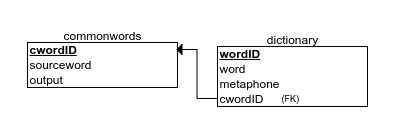
\includegraphics[scale=.65]{relational}
          \caption{Relational Diagram}
          \label{relational}
\end{figure}

\begin{figure}[H]
        \centering
          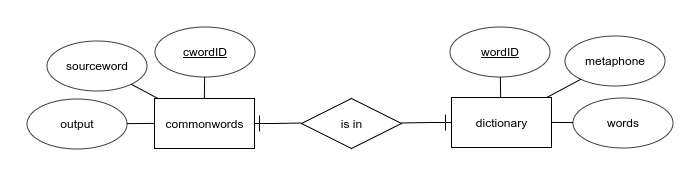
\includegraphics[scale=.50]{erd}
          \caption{ERD}
\end{figure}
\label{erd}
\begin{figure}
        \centering
          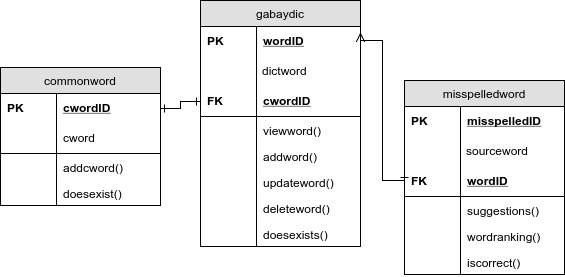
\includegraphics[scale=.75]{classdiagram}
          \caption{Class Diagram}
\end{figure}

\chapter{Schedule}

\begin{table}[ht]
\begin{center}
\begin{tabular}{|M{10cm}|M{5cm}|N}
 \hline
 \textbf{Activities} & \textbf{Due of Date}&\\[40pt]
 \hline
 Final Revision of Proposal & May 27-31 &\\[40pt]
 \hline
 Implementation & June to September&\\[40pt]
 \hline
 Gather Training Sets, Populate Database & October 1-12&\\[40pt]
 \hline
 Chapter 5: Evaluation; and Revision & October 13-20&\\[40pt]
 \hline
 Chapter 6: Discussion and Conclusion; and Revision & October 21-27&\\[40pt]
 \hline
 Overall Revision & November 12-16&\\[40pt]
 \hline
 Final Revision & November 17-2&\\[40pt]
 \hline
 Submission of Final Paper & November 26-30&\\[40pt]
 \hline
 
\end{tabular}
\end{center}
\caption{Research Schedule}
\end{table}

\clearpage
\pagebreak

\bibliographystyle{apacite}
\bibliography{References}
\end{document}